%!TEX root =../main-tokyo.tex
% ##################################################################################################################
\chapter{Tokyo: Simulating Hyperpath-based Vehicle Navigations and its Impact on Travel Time Reliability}
\label{ch:tokyo}
\hfill \textbf{Authors:} Daisuke Fukuda, Jiangshan Ma, Kaoru Yamada, Norihito Shinkai

% ##################################################################################################################
\section{Introduction}

Most of standard commercial vehicle navigation systems usually rely on fixed travel times as link weights while sophisticated algorithms mostly deals with stochastic travel time. Reliable routing considering such travel time variability would have a potential of providing extra benefits to drivers. However, implementations of many reliable routing algorithms might become intractable in practice mainly due to heavy computational loads. The hyperpath-based navigation demonstrated in this chapter would only consider lower and upper bounds travel times for each link as inputs and produces a set of potentially optimal links together with recommended link choice possibilities.  

The basic concept of hyperpath is that ``Do not put all eggs in one basket in an uncertain environment'' and so that the actual routes are more widely distributed as the congestion goes up. In this way, the risk of delay due to the induced congestion would become lower and the network burden in terms of congested links is expected to be reduced (Figure~\ref{fig:tokyo_fig1}). Based on the idea of ``Optimal strategy'' widely employed in frequency-based transit assignment \citep[see][]{Spiess1989}, \citet{Bell2009} proposed the shortest hyperpath search algorithm called ``Hyperstar''. Variant of algorithms under various conditions have been further developed in \citet{Bell2012} and \citet{Ma2013} for risk-averse vehicle navigation.

%------------
\createfigure%
{Concept of hyperpath under travel time uncertainty (1\,\gls{od} - 3\,routes example)}%
{Concept of hyperpath under travel time uncertainty (1\,\gls{od} - 3\,routes example)}%
{\label{fig:tokyo_fig1}}%
{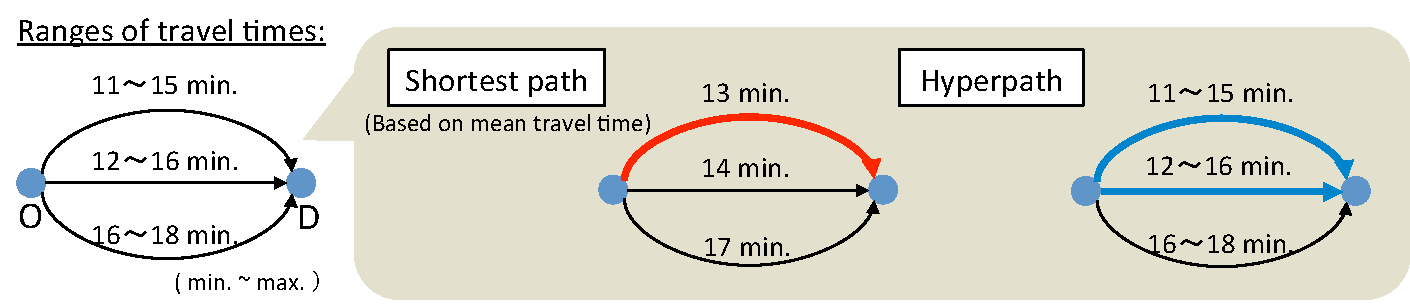
\includegraphics[width=0.90\textwidth, angle=0]{./scenarios/figures/tokyo_fig1.pdf}}%
{}
%------------

The hyperpath-based navigation is expected to be beneficial mainly in the following three aspects: 
\begin{enumerate}
\item The concept of hyperpath might be beneficial for drivers since it can help to reduce travel time unreliability by providing the opportunity of adaptive choices that potentially avoid stops at intersections or long delay on links to a certain extent. For example, differently to typical navigation systems, the turn notification received by drivers before entering intersections could be ``go straight or turn right''. In this case, drivers may decide to turn right when meeting with red signal for going straight. Even if the final experienced travel time is slightly longer than non-adaptive drive, the driving experience could be better (say, eight\,minutes driving plus two\,minutes waiting versus ten\,minutes non-stop driving).
\item For drivers hyperpath also could cater to more individual tastes without predefining drivers' actual route choice preferences. Comparatively, shortest path (SP) or multiple shortest paths with different criterion would require modelers' definition of ``shortest''. In the long run, the hyperpath model has the potential to evolve with reinforcement learning technologies and provide more customized adaptive route guidance.
\item Existing commercial navigation systems seldom take their effects on networks into consideration and sometimes congestion occurs for the reason of being actually induced by their navigation to many vehicles. Consequently, \gls{dta} along with route guidance might be still mostly in the field of academic research. Classical \gls{dta} are mostly based on time-dependent K-shortest paths and mostly aim to analyze equilibrium conditions as ideal states. For example, Dynamic User Equilibrium defines the equilibrium that drivers cannot change their trip plans to reduce actual experienced travel time. However, the experienced travel time can never be known beforehand since the real-life transportation is much more complicated than laboratory \gls{dta} settings. Hyperpath-based route choice does not chase for equilibrium but it might be equilibrium-like to some extent for being strategically reactive to the delay changes. 
\end{enumerate}

The hyperpath-based route recommendation thus would have the potential of reducing the congestion of the entire network because it recommends a potential optimal set of paths instead of the shortest (single) path and lead to the dispersion of traffic in an appropriate way. However, its impacts on the entire traffic networks have not been well analyzed. In this chapter we demonstrate how the market penetration of the hyperpath-based vehicle navigation would affect the entire network performances using \gls{matsim}.  Though the development of real-time traffic information for navigating vehicles has benefited drivers to some extent, the market diffusion of these technologies may not lead to the reduction of traffic congestion mainly due to the concentration of traffic into particular paths or links in the traffic networks. Some unexpected phenomena such as ``Hunting \citep[e.g.,][]{Oguchi2003}'' might happen. We change the ratio of vehicles with the risk-averse route guidance, conduct traffic simulation and then check the performance of the traffic.


\section{A Small-Sized Network Case}

\gls{matsim} is utilized as the simulation tool. In the early stage, we conducted such simulations on the Sioux Falls network (see also Chapter~\ref{ch:siouxfalls}) with synthetic \gls{od} demands. See \citep{Yamada2013} for the details. Hyperpath algorithm is initially written as an external route planning module in Python and the market share can be configured by setting the ``ModuleProbability'' item. Figure~\ref{fig:tokyo_fig2} illustrates the configuration sample for hyperpath with 20\,\% market share. Also, Figure~\ref{fig:tokyo_fig3} shows the network state (in terms of link speed) improvement with increase in the market share of hyperpath from 20\,\% to 80\,\%.

%------------
\createfigure%
{Setting for the case that 20 \% of vehicles follow hyperpath-based vehicle navigation}%
{Setting for the case that 20 \% of vehicles follow hyperpath-based vehicle navigation}%
{\label{fig:tokyo_fig2}}%
{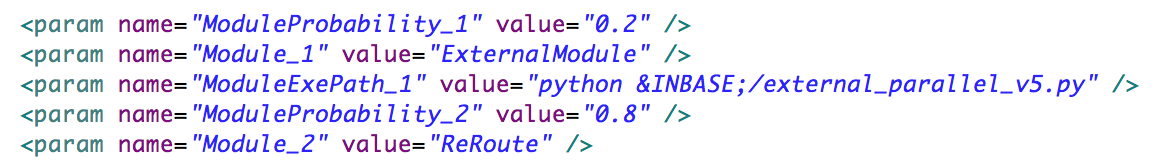
\includegraphics[width=0.95\textwidth, angle=0]{./scenarios/figures/tokyo_fig2.png}}%
{}
%------------

%------------
\createfigure%
{Link travel speeds for different levels of market penetrations}%
{Link travel speeds for different levels of market penetrations}%
{\label{fig:tokyo_fig3}}%
{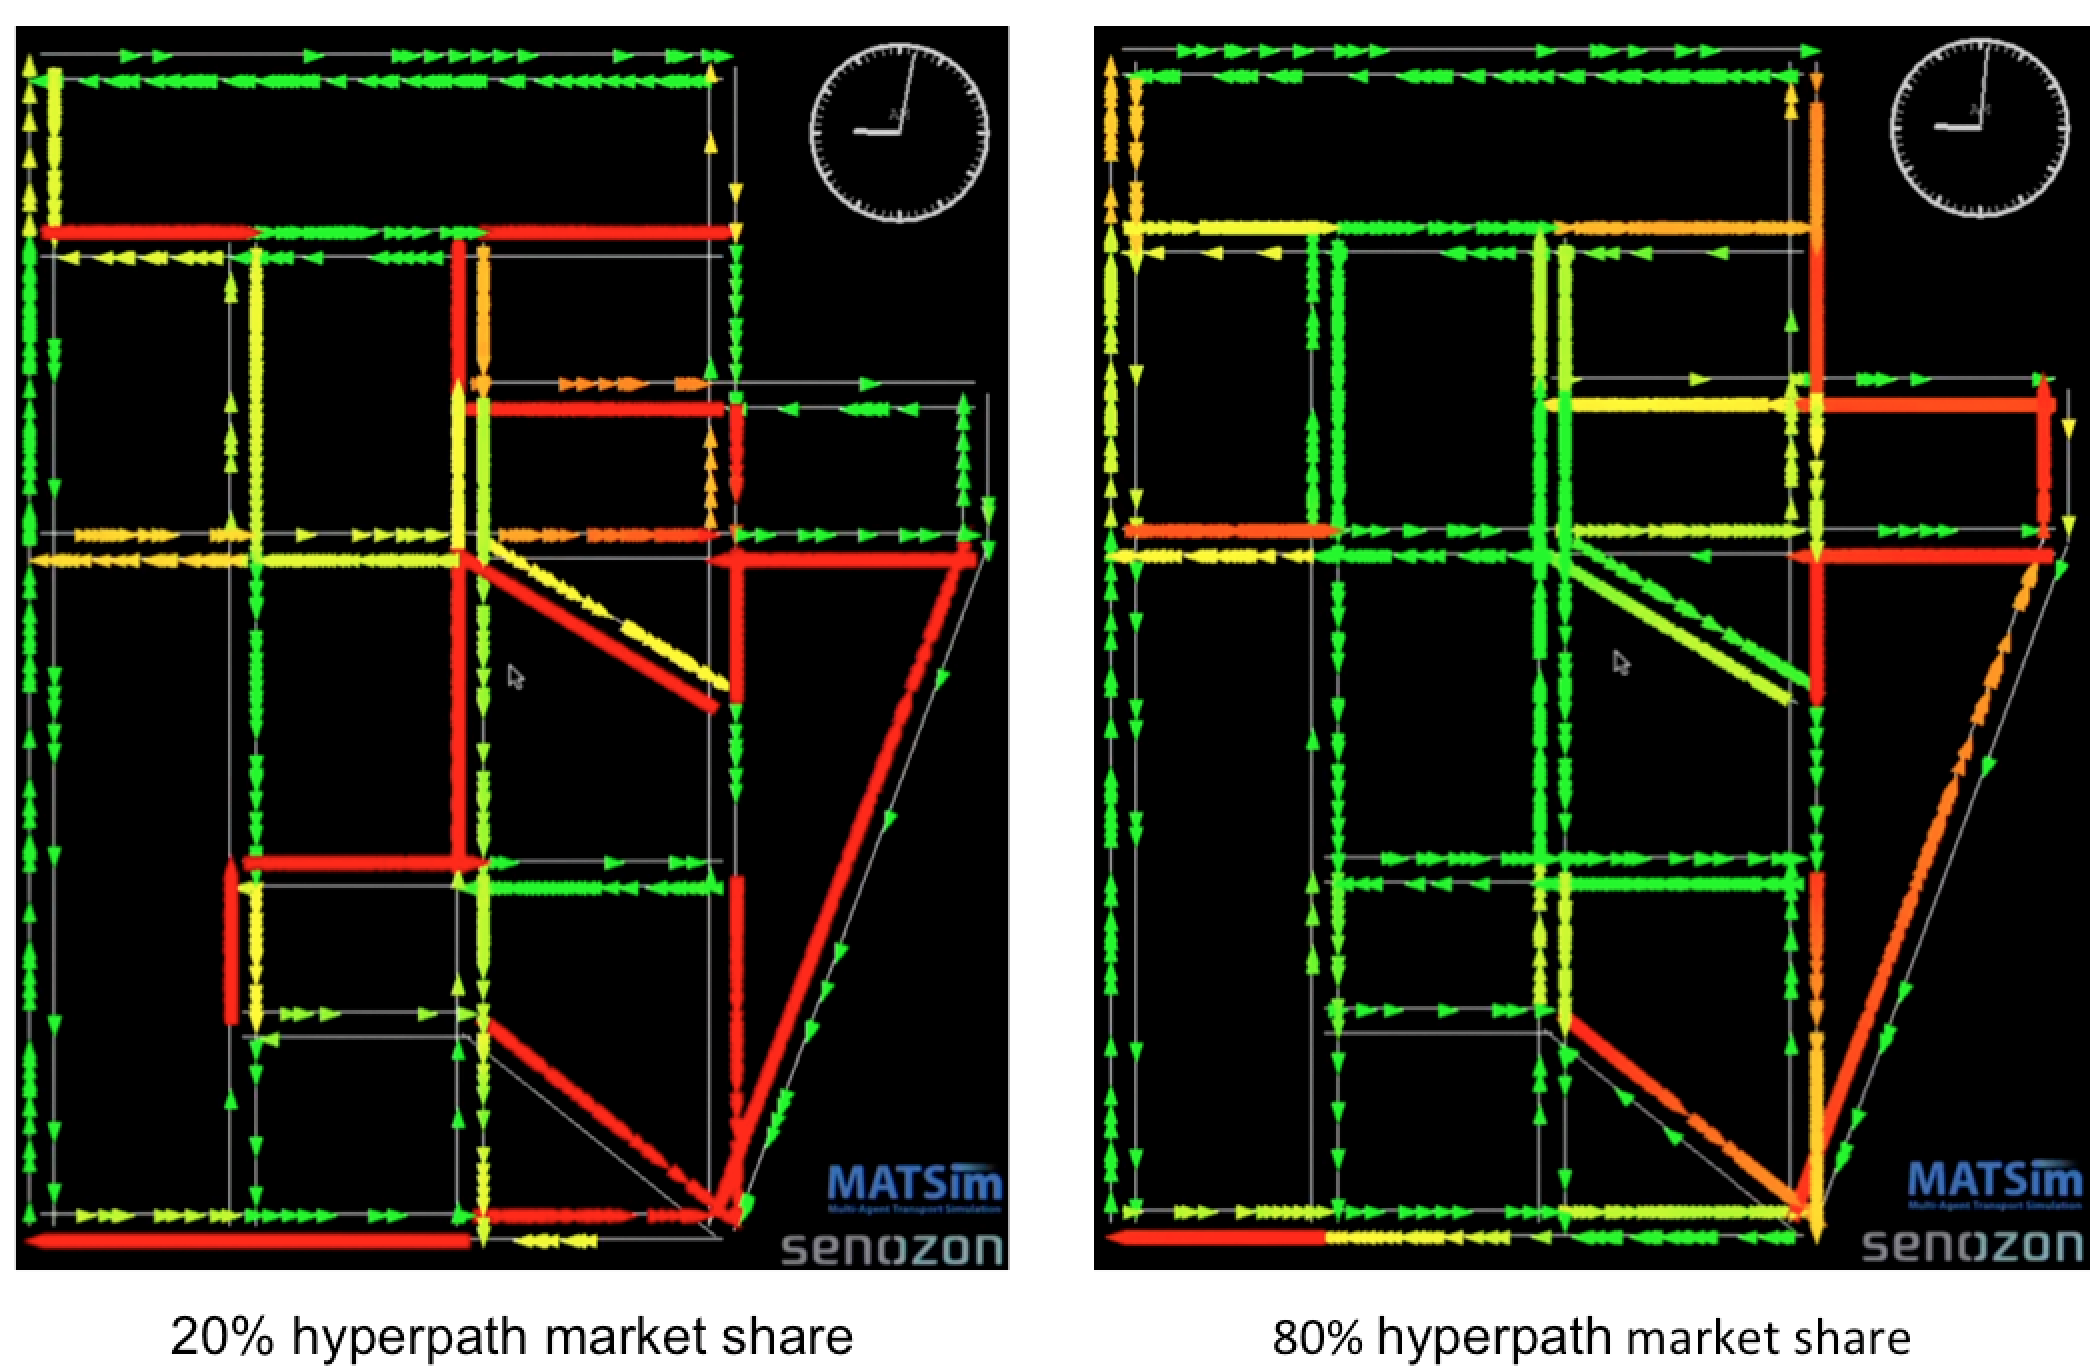
\includegraphics[width=0.85\textwidth, angle=0]{./scenarios/figures/tokyo_fig3.png}}%
{}
%------------


\section{Simulation in Tokyo's Arterial Road Network}
Based on the early-stage experiments on Sioux Falls network, we are interested in the similar simulation in Tokyo's large-scale arterial network with actual traffic data. 

\subsection{Network and Travel Demand}
The arterial road network including the whole Tokyo Metropolitan Area (Figure~\ref{fig:tokyo_fig4}) is prepared from Digital Road Map version~2011 (DRM2403) within the radius of about 70--80\,kilometer from the downtown. The traffic network consists 444\,220\,nodes and 177\,971\,links after being cleaned using the ``networkcleaner'' API in \gls{matsim}. Capacity and free flow speed of each link are setup by considering the information of road hierarchy, type of links and their corresponding speed limits. 

 %------------
\createfigure%
{Arterial road network in Tokyo Metropolitan Area}%
{Arterial road network in Tokyo Metropolitan Area}%
{\label{fig:tokyo_fig4}}%
{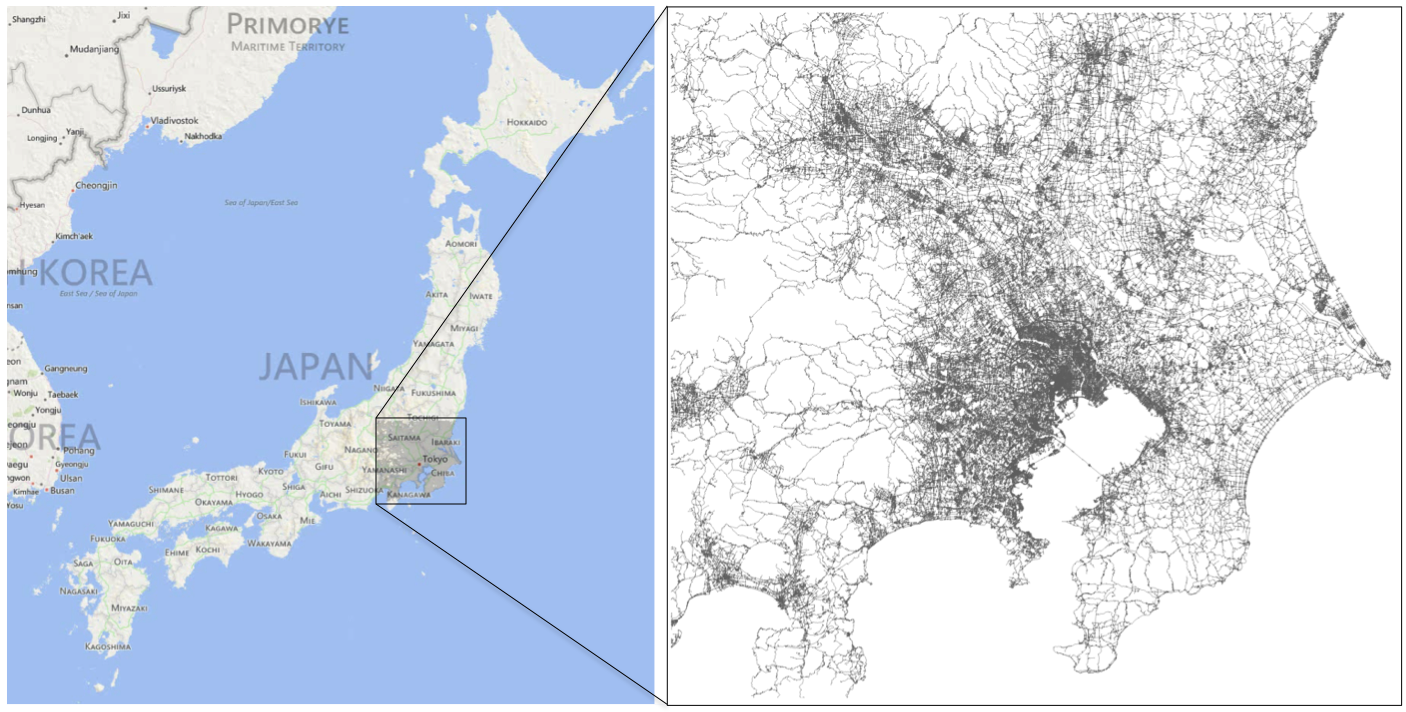
\includegraphics[width=0.90\textwidth, angle=0]{./scenarios/figures/tokyo_fig4.png}}%
{}
 %------------

We analyze car traffic during the period of morning rush hours and the \gls{od} table is subtracted from a large-scale travel survey (Person Trip Survey~2007) to create the agents' plans. The total number of the \gls{od} pairs is 17\,186 and there are about 2\,307\,000 vehicular trips during the target time period in the whole area. From the data, 219\,642 agents (approximately 10\,\% sampling rate) are randomly created and each agent has only one activity, which is the commuting activity from his/her home to the working place. Regarding the drivers' departure time from home, a normal distribution with the mean of 7\,AM and the standard deviation of 1\,hour was assumed.

\subsection{Setup of Day-to-Day Simulation Experiments}
Although the Logit-based route planning module has already been employed as one of the routing strategies in \gls{matsim}, it may have less supportive explanations in the sense of route guidance. We therefore focus on the combination of ``re-route'' and ``best-score'' planning modules, which means that some drivers adjust their daily travel plan according to yesterday's experience while the others simply choose the best experienced route from their past choices. 

To get travel time data for creating hyperpaths, simulation runs for 30\,iterations (\ie 30\,days) are firstly performed with no HP-based drivers (\ie 100\,\% of SP-based drivers) to obtain travel time distribution. Then, maximum delay of each during these 30\,days are computed and used in the following main simulation with the market diffusion of HP-based navigated drivers. Figure~\ref{fig:tokyo_fig5} illustrates a simulation with \gls{matsim} for the downtown of Tokyo. 

%------------
\createfigure%
{Snapshot of the hyperpath-based traffic simulation in Tokyo}%
{Snapshot of the hyperpath-based traffic simulation in Tokyo}%
{\label{fig:tokyo_fig5}}%
{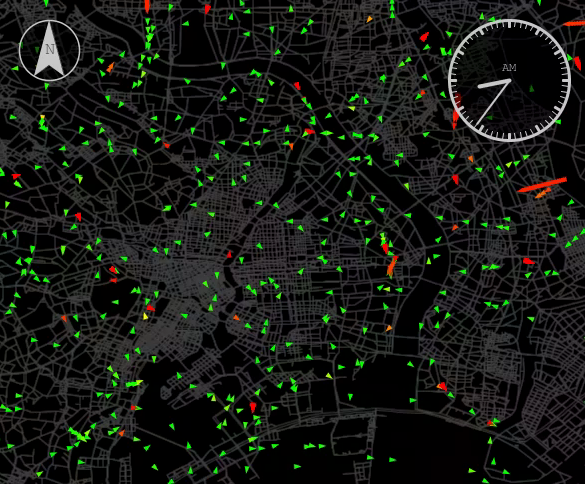
\includegraphics[width=0.68\textwidth, angle=0]{./scenarios/figures/tokyo_fig5.png}}%
{}
 %------------

\subsection{Results}
We conduct five different cases of traffic simulation by changing the shares of HP-based drivers from 0\% to 80\% by 20\%. The simulation runs are conducted for 30\,days for each case to evaluate network-level travel-time savings as well as reliability. 

The average travel time per unit length of the whole agents in each one day is plotted for different cases in Figure~\ref{fig:tokyo_fig6}. Since the traffic network in Tokyo is quite large and the trip lengths of drivers are diverse, we plot the average travel time per unit length (shortly ATTPUL) for the fair comparison. It seems that there are high levels and large fluctuations in ATTPUL for the case that there are no HP-based drivers (HP\,\%, that is SP 100\,\%). But it is obvious that as the market diffusion rate of HP-based drivers increase, not only the levels of ATTPUL but also the fluctuation of ATTPUL would significantly be reduced.


%------------
\createfigure%
{Average travel time per unit length for all vehicles}%
{Average travel time per unit length for all vehicles}%
{\label{fig:tokyo_fig6}}%
{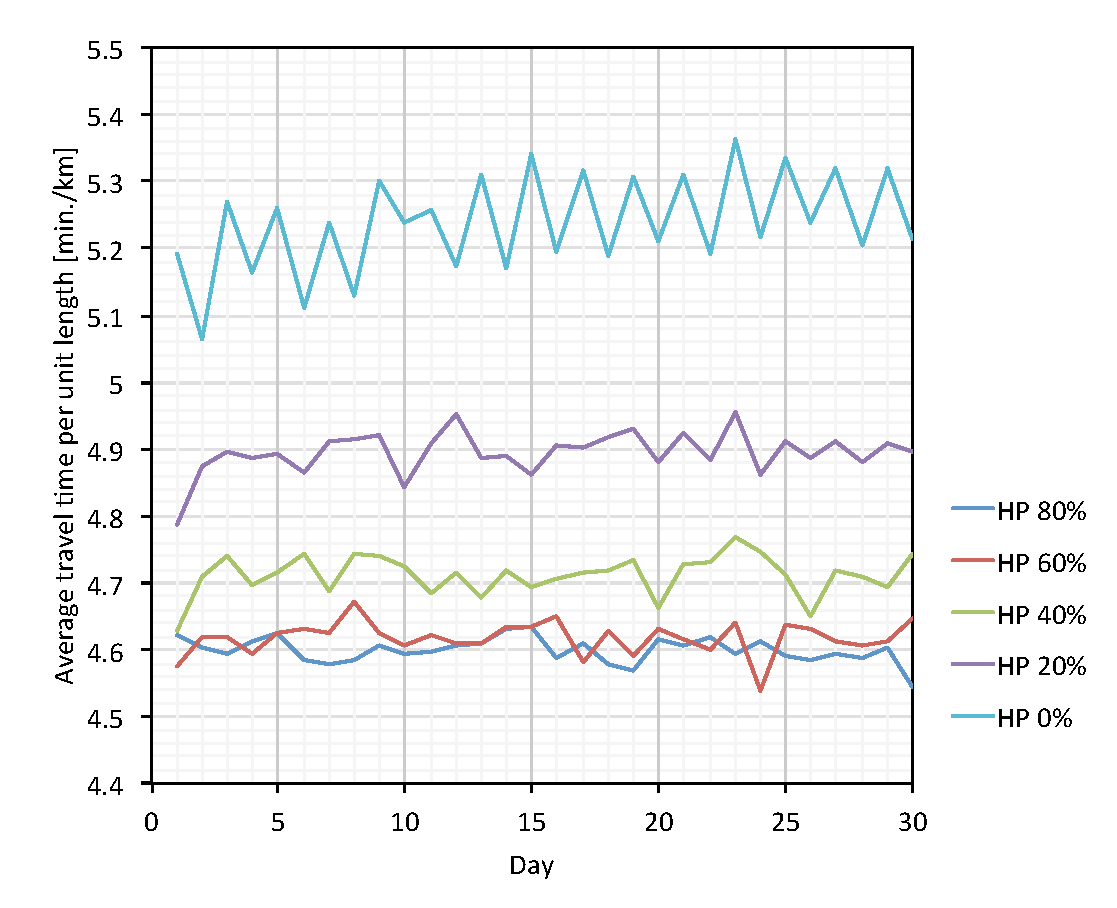
\includegraphics[width=0.70\textwidth, angle=0]{./scenarios/figures/tokyo_fig6.pdf}}%
{}
 %------------


Table~\ref{tab:tokyo_1} summarizes the result of Figure~\ref{fig:tokyo_fig6} by computing the average of the ATTPUL ($\overline{t}_{unit}$) as well as the standard deviation of the ATTPUL ($\sigma_{unit}$) over the 30\,days. It is clear from this table that both average and standard deviation of travel time has the decreasing tendency when the mixing ratio of HP-based route guidance is increased. This result indicates the possibility that HP-based route guidance would be superior from the viewpoint of travel time reduction as well as travel time reliability when observing the day-to-day patterns of average travel time for the heavy traffic demand in Tokyo. 

 %------------
\begin{table}[h]
		\small
		\caption{Summary of the network perfomance}
		\begin{tabular}{ccc}
			\hline
			Case & $\overline{t}_{unit}$ [min./km] & $\sigma_{unit}$ [min./km]\\
			\hline
			HP 80\%& 4.60& 0.02 \\
			HP 60\%& 4.62 & 0.02 \\
			HP 40\%& 4.71 & 0.03 \\
			HP 20\%& 4.90 & 0.03  \\
			HP 0\%& 5.24 & 0.07 \\
			\hline
		\end{tabular}
		\label{tab:tokyo_1}
\end{table}
 %------------

 
\section{Validation of Hyperpath-Based Navigation}
A field experiment has been conducted to verify the benefits of travel time reliability improvement for drivers by \citet{Ito2015} in Tokyo. Drivers equipped with the time-dependent shortest path and those who equipped the time-dependent hyperpath navigation systems have been compared. Both navigation systems use the same historical travel time sourced from probe vehicle data. Based on the results collected from two-week experimental driving by different drivers, the hyperpath shows a better off significantly, especially when the network is quite congested. 

% ##################################################################################################################